%! Author = itgramic
%! Date = 05.12.23

% Preamble
\clearpage
\subsubsection{Monolithische vs. verteilte SQL Systeme}
\begin{flushleft}
    Klassische SQL-Datenbanken sind monolithische Systeme, selbst wenn sie mit Hilfe Replikation eine Primary/Stand-by-Architektur aufweisen.
    Man kann mit eines SQL-Proxys ein gewisses Mass an Load Balancing betreiben, hat aber immer noch das Problem, das es einen primären Node gibt, auf dem beschrieben wird.
    Monolithische Systeme sind daher nicht Cloud Native.
\end{flushleft}
\begin{flushleft}
    Nur verteilte Systeme, sogenannte Distributed SQL Systeme, sind wirklich Cloud Native fähig,\\
    da die Last gleichmässig auf horizontal skalierenden Nodes verteilt werden kann.\\
    Nachfolgend die schematische Darstellung der beiden Konzepte:
    \begin{figure}[H]
        \centering
        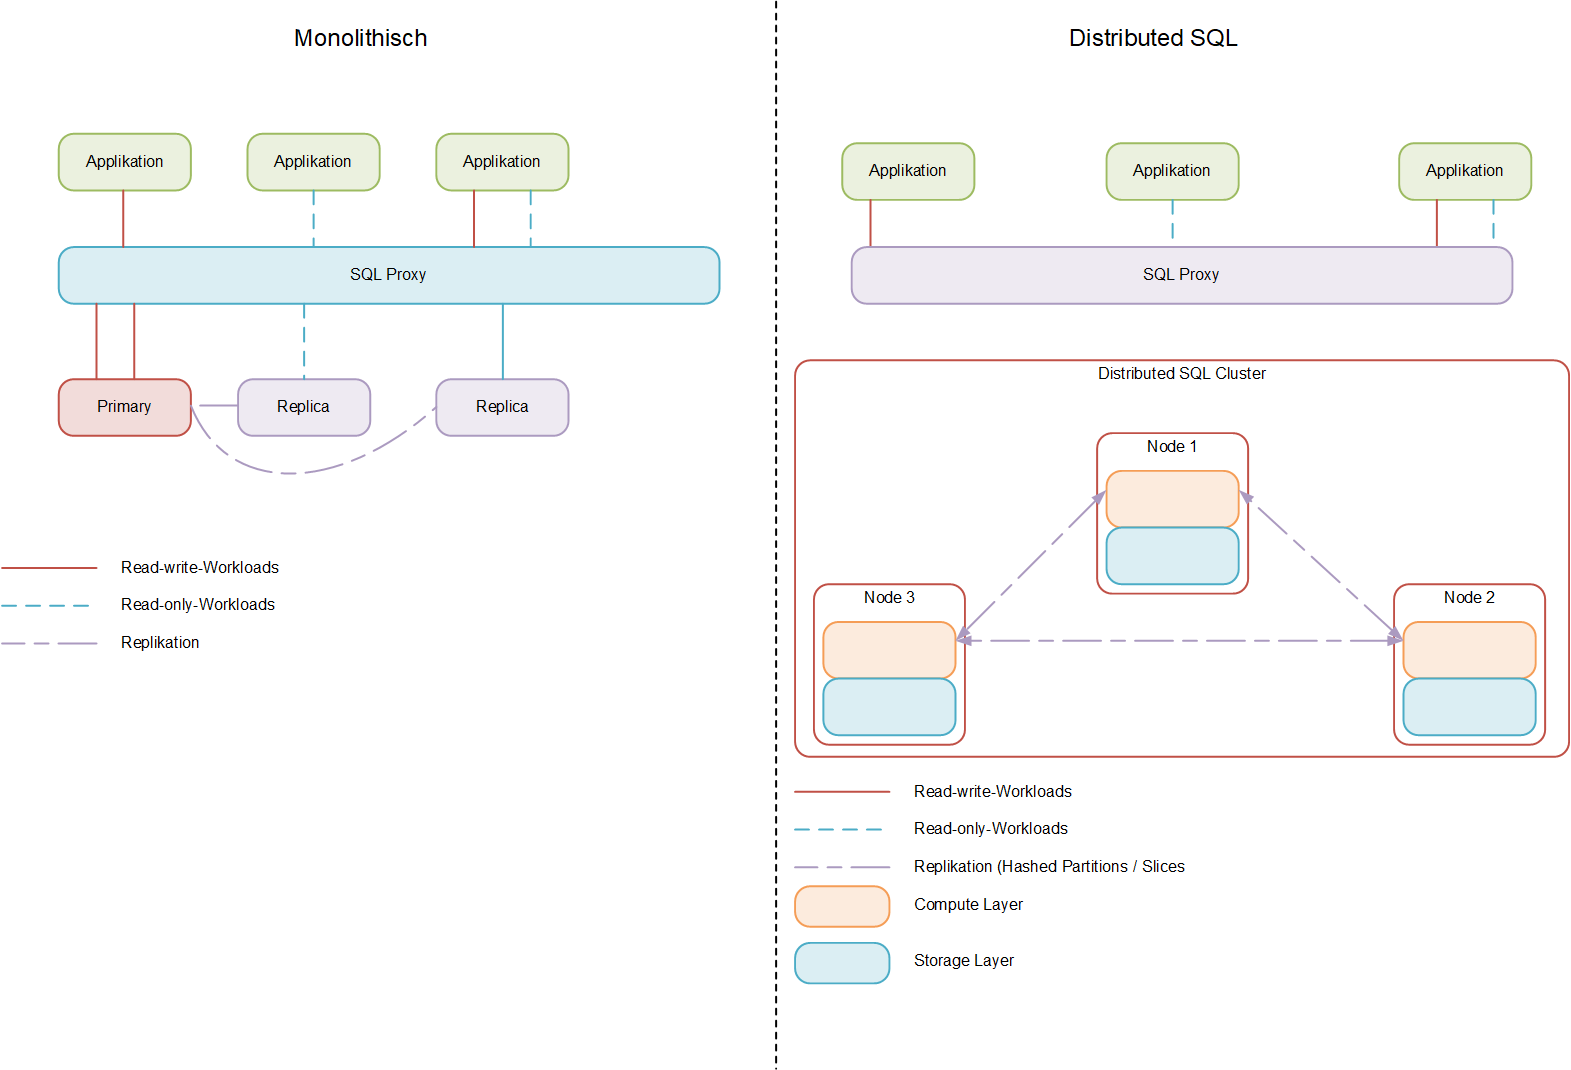
\includegraphics[width=1\linewidth]{source/implementation/evaluation/excursus_architecture/monolith_distributed}
        \caption{Monolithische vs. verteilte SQL Systeme}
        \label{fig:Monolith_vs_Distributed_SQL}
    \end{figure}
\end{flushleft}
